\documentclass[a4paper]{article}
\usepackage[left=1.5in,right=1.5in,bottom=1in]{geometry}

\usepackage{graphicx}
\usepackage[ngerman]{babel}
 \usepackage{fourier}
%\usepackage{venturis}
\usepackage[final,babel]{microtype}

\usepackage{todonotes}
\usepackage[colorlinks=true,urlcolor=blue]{hyperref}
\usepackage{transparent}
\usepackage{eso-pic}


\newcommand\marklessfootnote[1]{%
  \begingroup
  \renewcommand\thefootnote{}\footnote{#1}%
  \addtocounter{footnote}{-1}%
  \endgroup
}

%%%Background image:

\newcommand\backgroundimage{%
\put(0,0){%
\parbox[b][\paperheight]{\paperwidth}{%
\centering
{\transparent{0.4}%
  %
  %
  % Here you can insert the background image
  % and play around with width and height.
  % keepaspectratio will not distort the image but possibly display only part of it.
  % see also https://tex.stackexchange.com/questions/46280/how-to-create-a-background-image-on-title-page-with-latex
  %
  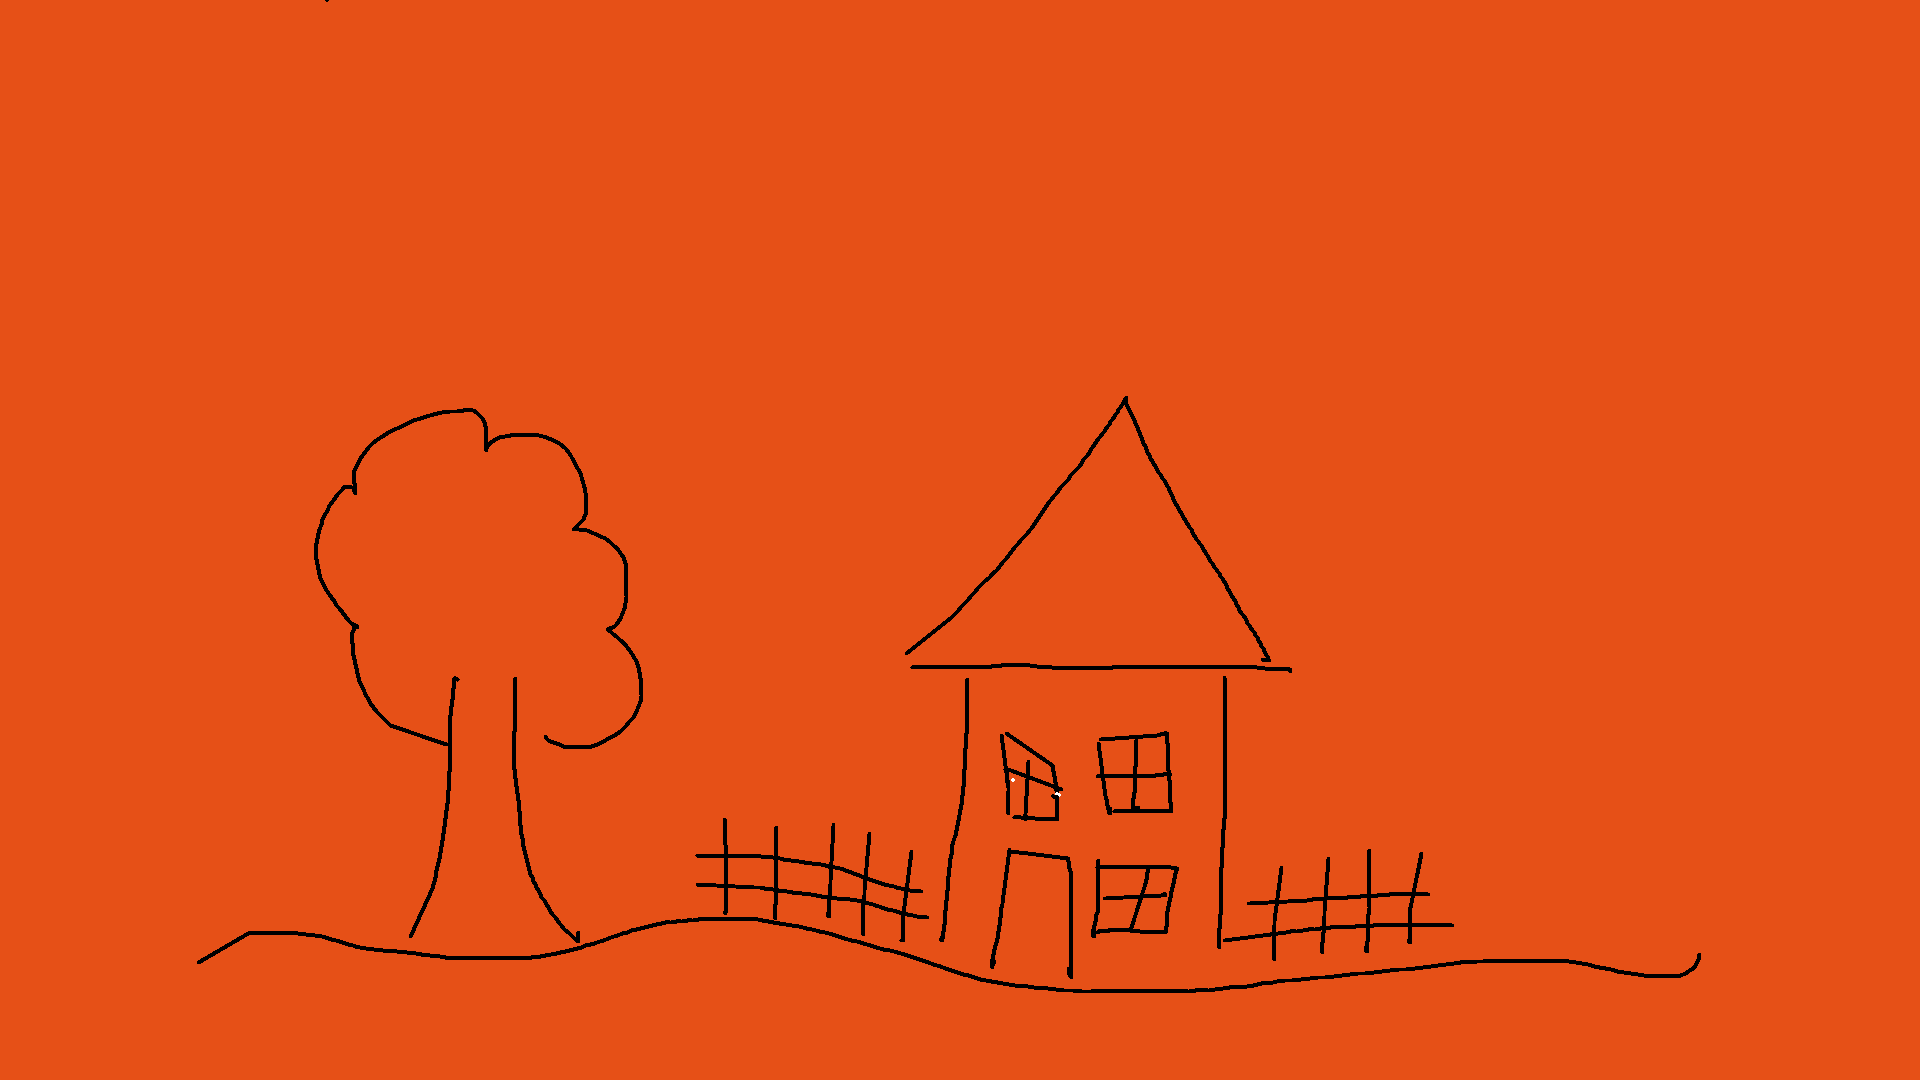
\includegraphics[% width=\paperwidth,
  height=\paperheight,%
  keepaspectratio]{background.png}}%
\vfill
}}}
\begin{document}
%%% needed for background image:
\AddToShipoutPicture*{\backgroundimage}

\thispagestyle{empty}

\section*{Studentische Hilfskraft gesucht}
Wir suchen eine wissenschaftliche Hilfskraft, um dies und das zu machen\footnote{\url{example.com}}\dots

\subsection*{Voraussetzungen sind:}
\begin{itemize}
\item Erfahrung in diesem und jenem
\end{itemize}

\subsection*{Wir bieten:}
\begin{itemize}
\item Ein Hiwi-Gehalt für bis zu $0.3$ Stunden.
\end{itemize}

\vspace{1cm}

\noindent Bei Interesse bitte bei Max Mustermann (\href{mailto:max.mustermann@example.com}{max.mustermann@example.com}) melden.

\vfill

\marklessfootnote{Bild von Erika Musterfrau}

\end{document}
